\documentclass[tikz,border=8pt]{standalone}
\usetikzlibrary{arrows.meta,positioning}
\begin{document}
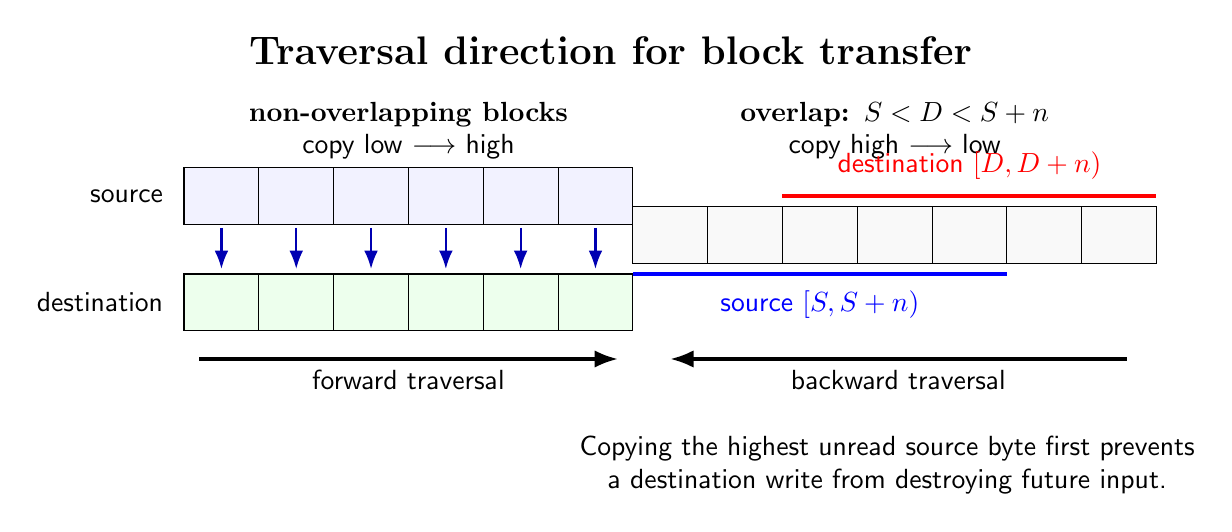
\begin{tikzpicture}[font=\sffamily,>=Latex,x=.95cm,y=.9cm]
\node[font=\Large\bfseries] at (6.2,7.1) {Traversal direction for block transfer};
\node[font=\bfseries] at (3.5,6.2) {non-overlapping blocks};
\node at (3.5,5.75) {copy low $\longrightarrow$ high};
\foreach \x in {0,...,5}{
  \fill[blue!5] (\x+.5,4.65) rectangle ++(1,.8);
  \fill[green!7] (\x+.5,3.15) rectangle ++(1,.8);
  \draw (\x+.5,4.65) rectangle ++(1,.8);
  \draw (\x+.5,3.15) rectangle ++(1,.8);
  \draw[blue!70!black,thick,->] (\x+1,4.6)--(\x+1,4.02);
}
\node[left] at (.35,5.05) {source};
\node[left] at (.35,3.55) {destination};
\draw[very thick,->] (.7,2.75)--(6.3,2.75) node[midway,below] {forward traversal};

\node[font=\bfseries] at (10.0,6.2) {overlap: $S<D<S+n$};
\node at (10.0,5.75) {copy high $\longrightarrow$ low};
\foreach \x in {0,...,6}{\fill[gray!5] (\x+6.5,4.1) rectangle ++(1,.8); \draw (\x+6.5,4.1) rectangle ++(1,.8);}
\draw[very thick,blue] (6.5,3.95)--(11.5,3.95) node[midway,below=2pt] {source $[S,S+n)$};
\draw[very thick,red] (8.5,5.05)--(13.5,5.05) node[midway,above=2pt] {destination $[D,D+n)$};
\draw[very thick,->] (13.1,2.75)--(7.0,2.75) node[midway,below] {backward traversal};
\node[align=center] at (9.9,1.25) {Copying the highest unread source byte first prevents\\a destination write from destroying future input.};
\end{tikzpicture}
\end{document}
